\documentclass[12pt,a4paper]{beamer}
% \usepackage{amsmath}
% \usepackage{amsfonts}
% \usepackage{amssymb}
\usepackage{graphicx}
\usepackage{hyperref}
\usepackage{lmodern}
\usepackage{listings}
\usepackage[utf8x]{inputenc}
\usepackage[L7x]{fontenc}
\usepackage[lithuanian]{babel}

\usetheme{Antibes} 
\usecolortheme[RGB={155,192,12}]{structure} 

\author{Povilas Balzaravičius}
\title{Seni projektai, nauji įrankiai}
\subtitle{VilniusPHP Susitikimas \#1}

\begin{document}
\begin{frame}
	\titlepage
\end{frame}

\section{Įžanga}
\begin{frame}{Kas aš toks?}
    \begin{itemize}
        \item Povilas Balzaravičius
        \item \href{https://twitter.com/pawka}{@Pawka}
        \item \href{https://github.com/pawka}{github.com/pawka}
        \item \href{https://linkedin.com/in/pawka}{linkedin.com/in/pawka}
        \item \href{http://pawka.linija.net}{pawka.linija.net}
    \end{itemize}
    \begin{center}
        
\includegraphics[scale=0.4]{img/estina.png}
        \hskip1cm
        
\includegraphics[scale=0.4]{img/zce-php5-3-logo.png}
    \end{center}
\end{frame}

\subsection{Seni projektai}
\begin{frame}[fragile]

    {\Huge Seni projektai}
\end{frame}

\begin{frame}{Kas jie tokie?}
    \begin{itemize}
        \item PHP 4.x/5.x.
        \item Kodas >= 4 metų senumo.
        \item Niekur nematytas kodo stilius(-ai).
        \item Nenaudojamas žmonijai žinomas karkasas.
        \item \textbf{include}, \textbf{require} ir draugai.
    \end{itemize}
\end{frame}

\begin{frame}{Kylančios problemos}
    \begin{itemize}
        \item Didžiulės sąnaudos tvarkingai perrašyti kodą.
        \item Naujo funkcionalumo pridėjimas reikalauja daug laiko.
        \item Šlykštoka dirbti\dots
    \end{itemize}
\end{frame}

\section{Projektų gaivinimas}

\subsection{Kodo stilius}
\begin{frame}

    {\Huge Stilius}\\
    Naujas projektas - naujas programavimo stilius.
\end{frame}

\begin{frame}[fragile]
    \frametitle{Standartas}

    {\Huge PSR}
\end{frame}

\begin{frame}
    \frametitle{PSR Standartas}
    {\large PHP Specification Request - programavimo stiliaus rekomendacija.}
    \vskip15pt
    \pause
    Sudaro trys dokumentai:
    \begin{description}
        \item[PSR-0] Autoload standartas.
        \pause
        \item[PSR-1] ``Basic Coding Standard'' - Koduotė, PHP \textit{tagai}, konstantos, klasių ir metodų pavadinimai, \dots
        \pause
        \item[PSR-2] ``Coding Style Guide'' - Tarpai, skliausteliai ir kableliai :-)
        \pause
    \end{description}
    \vskip10pt
    {\small Standarto aprašymas: \href{https://github.com/php-fig/fig-standards/}{github.com/php-fig/fig-standards/}}
\end{frame}

\begin{frame}[fragile]
    \frametitle{Sprendimas}

    {\Huge php-cs-fixer}
\end{frame}

\begin{frame}
    \frametitle{PHP Coding Standards Fixer}
    Įrankis skirtas kodo stiliaus tvarkymui pagal \textbf{PSR-1} ir \textbf{PSR-2} standartus.
    \begin{itemize}
        \item Autorius: Fabien Potencier
        \item \url{http://cs.sensiolabs.org/}
        \item Galimybė tvarkyti tik tam tikras sritis (identacija, skliaustų išdėstymas, \dots)
        \item \dots ir/arba naudoti paruoštas konfigūracijas (sf20, sf21, magento, default).
    \end{itemize}
\end{frame}

\begin{frame}
    \frametitle{PHP Coding Standards Fixer - naudojimas}
    {\small
        \begin{enumerate}
            \item sudo wget http://cs.sensiolabs.org/get/php-cs-fixer.phar -O /usr/local/bin/php-cs-fixer
            \item sudo chmod a+x /usr/local/bin/php-cs-fixer
            \item php php-cs-fixer.phar fix /path/to/dir
            \item Džiaugiamės tvarkingu kodu :-) \pause(dažniausiai)
        \end{enumerate}
    }
\end{frame}
% TODO - add console sceenshot.

\subsection{Išorinės bibliotekos}
\begin{frame}[fragile]

    {\Huge Išorinės bibliotekos}
\end{frame}

\begin{frame}
    \frametitle{Problemos}
    \begin{itemize}
        \item Nepatogu įtrauktį į kodą.
        \item Gali priklausyti nuo kitų bibliotekų.
        \item Saugomos kartu su projekto kodu.
        \item Nepatogu atnaujinti.
    \end{itemize}
\end{frame}

\begin{frame}[fragile]
    \frametitle{Sprendimas}

    {\Huge Composer}
\end{frame}

\begin{frame}
    \frametitle{Composer}

    \begin{itemize}
        \item Autorius: Jordi Boggiano
        \item \url{http://getcomposer.org/}
        \item Suranda, instaliuoja, atnaujina ir \textit{autoloadina} paketus.
    \end{itemize}
\end{frame}

\begin{frame}
    \frametitle{Composer - naudojimas}
        \begin{enumerate}
            \item curl -s https://getcomposer.org/installer | php 
            \item Parsiunčiamas {\color{orange}composer.phar}
            \item {\color{orange}php composer.phar <komanda>}
        \end{enumerate}
\end{frame}

\begin{frame}
    \frametitle{Composer - paketų instaliavimas}

    \begin{enumerate}
        \item Susirandam paketą ir jo versiją:\\{\color{orange}php composer.phar search kažkas} arba \url{packagist.org}.
        \item Pvz. \textbf{doctrine/dbal 2.3.0}.
        \item Įtraukiam paketą į \textbf{composer.json}.
        \item {\color{orange}php composer.phar install} (arba {\color{orange}update}).
        \item Parsiųs paketus ir sugeneruos Autoload failus.
    \end{enumerate}
\end{frame}

\begin{frame}
    \frametitle{Composer - naudojimas}

    composer.json pavyzdys
    \begin{center}
        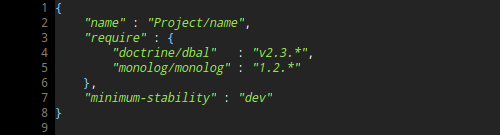
\includegraphics[scale=0.5]{img/composer_json.png}
    \end{center}
    \pause
    O tada\dots\\
    \begin{center}
        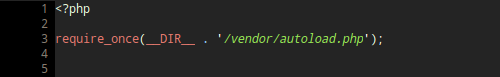
\includegraphics[scale=0.5]{img/autoload.png}
    \end{center}
\end{frame}


\begin{frame}[fragile]

    {\Huge Iš ko rinktis?}
\end{frame}

\begin{frame}
    \frametitle{Symfony Components}
    \url{symfony.com/components}
    {\scriptsize
        \begin{columns}[t]
            \begin{column}{5cm}
                \begin{itemize}
                    \item BrowserKit
                    \item ClassLoader
                    \item Config
                    \item Console
                    \item CssSelector
                    \item DependencyInjection
                    \item DomCrawler
                    \item EventDispatcher
                    \item Finder
                    \item Form
                    \item HttpFoundation
                \end{itemize}
            \end{column}
            \begin{column}{5cm}
                \begin{itemize}
                    \item HttpKernel	
                    \item Locale	
                    \item Process	
                    \item Routing	
                    \item Security	 	
                    \item Serializer	 	
                    \item Templating	
                    \item Translation	 	
                    \item Validator	 	
                    \item Yaml
                \end{itemize}
            \end{column}
        \end{columns}
    }
\end{frame}
\begin{frame}
    \frametitle{Zend Framework 2}

    {\Huge 48 atskiri komponentai}\\
    \url{framework.zend.com}
\end{frame}

\end{document}
